\documentclass[]{article}
\usepackage{lmodern}
\usepackage{amssymb,amsmath}
\usepackage{ifxetex,ifluatex}
\usepackage{fixltx2e} % provides \textsubscript
\ifnum 0\ifxetex 1\fi\ifluatex 1\fi=0 % if pdftex
  \usepackage[T1]{fontenc}
  \usepackage[utf8]{inputenc}
\else % if luatex or xelatex
  \ifxetex
    \usepackage{mathspec}
  \else
    \usepackage{fontspec}
  \fi
  \defaultfontfeatures{Ligatures=TeX,Scale=MatchLowercase}
\fi
% use upquote if available, for straight quotes in verbatim environments
\IfFileExists{upquote.sty}{\usepackage{upquote}}{}
% use microtype if available
\IfFileExists{microtype.sty}{%
\usepackage{microtype}
\UseMicrotypeSet[protrusion]{basicmath} % disable protrusion for tt fonts
}{}
\usepackage[margin=1in]{geometry}
\usepackage{hyperref}
\PassOptionsToPackage{usenames,dvipsnames}{color} % color is loaded by hyperref
\hypersetup{unicode=true,
            pdftitle={Plant-pollinator specialization: Origin and measurement of curvature},
            colorlinks=true,
            linkcolor=blue,
            citecolor=blue,
            urlcolor=blue,
            breaklinks=true}
\urlstyle{same}  % don't use monospace font for urls
\usepackage{longtable,booktabs}
\usepackage{graphicx,grffile}
\makeatletter
\def\maxwidth{\ifdim\Gin@nat@width>\linewidth\linewidth\else\Gin@nat@width\fi}
\def\maxheight{\ifdim\Gin@nat@height>\textheight\textheight\else\Gin@nat@height\fi}
\makeatother
% Scale images if necessary, so that they will not overflow the page
% margins by default, and it is still possible to overwrite the defaults
% using explicit options in \includegraphics[width, height, ...]{}
\setkeys{Gin}{width=\maxwidth,height=\maxheight,keepaspectratio}
\IfFileExists{parskip.sty}{%
\usepackage{parskip}
}{% else
\setlength{\parindent}{0pt}
\setlength{\parskip}{6pt plus 2pt minus 1pt}
}
\setlength{\emergencystretch}{3em}  % prevent overfull lines
\providecommand{\tightlist}{%
  \setlength{\itemsep}{0pt}\setlength{\parskip}{0pt}}
\setcounter{secnumdepth}{0}
% Redefines (sub)paragraphs to behave more like sections
\ifx\paragraph\undefined\else
\let\oldparagraph\paragraph
\renewcommand{\paragraph}[1]{\oldparagraph{#1}\mbox{}}
\fi
\ifx\subparagraph\undefined\else
\let\oldsubparagraph\subparagraph
\renewcommand{\subparagraph}[1]{\oldsubparagraph{#1}\mbox{}}
\fi

%%% Use protect on footnotes to avoid problems with footnotes in titles
\let\rmarkdownfootnote\footnote%
\def\footnote{\protect\rmarkdownfootnote}

%%% Change title format to be more compact
\usepackage{titling}

% Create subtitle command for use in maketitle
\providecommand{\subtitle}[1]{
  \posttitle{
    \begin{center}\large#1\end{center}
    }
}

\setlength{\droptitle}{-2em}

  \title{Plant-pollinator specialization: Origin and measurement of curvature}
    \pretitle{\vspace{\droptitle}\centering\huge}
  \posttitle{\par}
    \author{}
    \preauthor{}\postauthor{}
    \date{}
    \predate{}\postdate{}
  

\begin{document}
\maketitle

\hypertarget{to-do}{%
\paragraph{TO DO}\label{to-do}}

-table s2, sample sizes -reformat table s3 -pollinator diversification
in intro -incorporate ailene edits -incorporate tiago edits -read
Macleod 2002

\hypertarget{acknowledgements}{%
\paragraph{Acknowledgements}\label{acknowledgements}}

Sections 2, 3, and 4 were generously reviewed and improved by T.
Carvalho, A. MacPherson, and J.S. Légaré, respectively. M. Boehm was
funded by The University of British Columbia, and the Natural Sciences
and Engineering Research Council of Canada (NSERC). Q. Cronk was funded
by NSERC grant \#\ldots{}

\hypertarget{abstract}{%
\paragraph{Abstract}\label{abstract}}

The curvature of flowers and pollinator mouthparts (e.g.~hummingbird
bills) along the lateral plane is a widespread, convergent trait with
important ecological and evolutionary implications. Pollination
ecologists are concerned with flower-pollinator curvature because it
appears to be a derived trait associated with specialization,
competition, and species co-existence. In this review we summarize and
evaluate the methods historically used to measure curvature and suggest
a clarification of its definition by referring to the differential
geometry literature. Intuitively, curvature is the degree to which a
line is not straight, or more formally, the rate at which the unit
derivative changes direction with respect to arc length. To apply this
definition we suggest a protocol wherein a line is regressed against
landmarks placed on a lateral image of an organism, then computing
curvature at many points along the fitted line and taking the sum. This
protocol is demonstrated here by studying the development of nectar spur
curvature in \emph{Epimedium} (Berberidaceae). By clarifying the
definition of curvature, the language of comparitive morphology is made
more precise. In this study we found \emph{Epimedium koreanum} to have
an order of magnitude greater curvature than the closely related
\emph{E. grandiflorum} and \emph{E. violaceum}. This is to say that
\emph{E. koreanum} had greater total degrees of rotation along the arc
of the nectar spur. The functions used to quantify floral curvature in
this study are available as an open-source R package `curvy'. The major
advantages of this method are 1) precision of measurement is increased
without introducing expensive field equipment or computing power, 2)
precision of terminology within pollination ecology is improved by
adopting the existing mathematical lexicon for studying line-curves.

\hypertarget{the-ecology-of-flower-pollinator-curvature}{%
\paragraph{1. The ecology of flower-pollinator
curvature}\label{the-ecology-of-flower-pollinator-curvature}}

\begin{quote}
``We are beginning to understand why some hummingbird bills are long,
whereas others are short, and why some hummingbird flowers are wide,
whereas others are narrow. Now, why are bills of some hummingbirds and
the tubes of the flowers they visit curved?'' -- Temeles
(\protect\hyperlink{ref-temeles_1996}{1996}).
\end{quote}

At the center of plant-pollinator diversification is a remarkable
variety of floral form. The notion that plant communities experience
selection to reduce interspecific mating (``floral isolation'', Grant,
\protect\hyperlink{ref-grant_1949}{1949}) points to the importance of
floral diversity in initiating and reinforcing reproductive isolation
(Armbruster and Muchhala,
\protect\hyperlink{ref-armbruster_2009}{2009}). For example, in the
rapid radiation of Andean \emph{Centropogon} (Campanulaceae),
competition for pollination led to the divergence of floral traits
associated with bat and hummingbird pollination (Lagomarsino and
Muchhala, \protect\hyperlink{ref-lagomarsino_2019}{2019}). In the case
of South African \emph{Lapeirousia} (Iridaceae), geographic variation in
floral tube length has initiated reproductive isolation between morphs
with short and long corolla tubes, despite sharing the same fly
pollinator (Minnaar et al., \protect\hyperlink{ref-minnaar_2019}{2019}).
Patterns of plant-pollinator evolution point to both contemporaneous and
asymmetrical diversification (Cardinal and Danforth,
\protect\hyperlink{ref-cardinal_2013}{2013}; Tripp and McDade,
\protect\hyperlink{ref-tripp_2013}{2013}). In either case, floral
morphology is a key phenotype associated with the diversification of
plants and pollinators (Kay and Sargent,
\protect\hyperlink{ref-kay_2009}{2009}; Niet and Johnson,
\protect\hyperlink{ref-vanderniet_2012}{2012}; Ollerton,
\protect\hyperlink{ref-ollerton_2017}{2017}).

Flower-pollinator curvature as viewed from the side (lateral plane), has
been a trait of special interest since the post-Darwin era of
pollination ecology. In making pollinator observations of the Cape
flora, Scott-Elliott (\protect\hyperlink{ref-scott-elliot_1890}{1890})
noticed that the flowers of \emph{Leonotis ocymifolia} (Lamiaceae)
visited by \emph{Nectarinia} sunbirds were ``curved with the same
curvature as that of the bird's beak.'' (p.~272). Robertson
(\protect\hyperlink{ref-robertson_1889}{1889}) insightfully notes that
the curved nectar spurs of \emph{Viola} spp. (Violaceae) ``serves to
limit the insect visits much more than the mere length of the spur.''
(p.~172). From these early observations curvature has been synonymous
with specialization; we expect curvature to limit the range of
functional taxa in a plant-pollinator mutualism and strengthen
interactions between the existing participants. And these expectations
have largely been supported: Stiles
(\protect\hyperlink{ref-stiles_1975}{1975}) first posited that
neotropical \emph{Heliconia} partition hummingbird visitation by
flower-bill curvature, and that specialization by curve-billed
hummingbirds allow co-existence within the species-rich \emph{Heliconia}
clade. Subsequent research supports this hypothesis (Maglianesi et al.,
\protect\hyperlink{ref-maglianesi_2014}{2014}): along the slopes of the
Central Cordillera (Costa Rica), the degree of flower-hummingbird bill
curvature is proportional to plant-pollinator interaction strength
(Dehling et al., \protect\hyperlink{ref-dehling_2014}{2014}) and extent
of specialization (\emph{d'}, (Blüthgen et al.,
\protect\hyperlink{ref-bluthgen_2006}{2006}). More recently the scope of
plant-pollinator research has expanded to address the biogeography of
curvature. As predicted by Stiles
(\protect\hyperlink{ref-stiles_2004}{2004}), Maglianesi
(\protect\hyperlink{ref-maglianesi_2015_b}{2015}) and Sonne
(\protect\hyperlink{ref-sonne_2019}{2019}) find curvature to be most
prevalent in the lowland environments of the neotropics. Explanations
for this pattern range from heightened competition at lower elevations
to environmental filtering in the Andean highlands (Stiles,
\protect\hyperlink{ref-stiles_2004}{2004}; Graham et al.,
\protect\hyperlink{ref-graham_2009}{2009}). Because the neotropical
subfamily Phaethornithinae comprises the majority of hummingbird species
with curved bills, we might expect plant-hummingbird curvature to have a
predictable global distribution. In the case of honeycreepers and
honeyeaters and sunbirds ???

-Curvature and niche partitioning: -evidence that curvature is
correlated with a shift from insectivory to nectivory in hawaiin
honeycreepers (Carothers, \protect\hyperlink{ref-carothers_1982}{1982}).
-honeyeaters take longer to feed and intake less nectar on
experimentally curved flowers (Collins,
\protect\hyperlink{ref-collins_2008}{2008}) -aussie honeyeaters with
curved bills tend to be small nectivores and aerial insectivores rather
than stout-billed ground foragers. -see: wolf 1972 (Science), 1975
(Ecology)

Pollinator specialization has major effects on macroevolutionary and
biogeographic patterns (Kay and Sargent,
\protect\hyperlink{ref-kay_2009}{2009}; Armbruster and Muchhala,
\protect\hyperlink{ref-armbruster_2009}{2009}; Vamosi et al.,
\protect\hyperlink{ref-vamosi_2018}{2018}), and curvature is a
component, but widespread feature of specialist systems. Therefore, to
synthesize our knowledge of curved plant-pollinator systems, curvature
is a concept that needs an exact definition and method of measurement.
In the following section we summarize the approaches to measuring
curvature within the field of bird pollination, identify strengths and
shortcomings, and offer a solution with the aim of improving the
precision with which curvature is measured within the field of
pollination ecology. Although this review is motivated by the problem of
measuring curvature in plant-hummingbird systems, the solution is
general to any biological form modelled as a line curve: this case is
hopefully made in the demonstration to follow.

\hypertarget{summary-of-the-literature}{%
\paragraph{2. Summary of the
literature}\label{summary-of-the-literature}}

We searched the scientific literature for studies focusing on or
considering the curvature of flowers and their pollinators - a trait
commonly measured as a proxy for specialization. We make the distinction
between measuring curvature (e.g.~of petals) in the lateral plane versus
the curvature of surfaces. While lateral images are analysed for
line-curvature, images of specimens in the transverse plane can be used
to analyse surface (Gaussian) curvature (Nath et al.,
\protect\hyperlink{ref-nath_2003}{2003}; Coen and Rebocho,
\protect\hyperlink{ref-coen_2016}{2016}). The methods used in the latter
are relatively more complex, and perhaps because of this, comparitively
well-defined. At present, surface curvature has yet to be considered in
the context of pollination. However, because line and surface curvature
are related mathematical concepts, it will benefit pollination research
to clarify the simplest case (lines), with the goal of generating
interest in related ideas including the curvature of surfaces.

The literature was sourced by querying Web of Science and Google Scholar
for a topic search of (curv*) AND (pollinat*) AND (flower OR corolla OR
*bird OR *bee OR moth OR *fly). The initial search returned over 300
studies that were then screened for those that measured flowers and/or
animal mouthparts (e.g.~bird bills, moth tongues). We sorted studies
based on the criteria that 1) the study focused on pollination,
including qualitative measures of curvature and 2) the study measured
flower or animal (mouthpart) curvature for other reasons, but
measurements must be quantitative. 44 pollination studies were found
using some form of curvature metric (Table 1). An additional 11
publications discussing curvature, but not related to pollination are
included in Table S1. There were numerous studies of plant-pollinator
morphology that did not address curvature - these were omitted.

The first dedicated discussion of lateral curvature in plant-pollinator
interactions begins with Hainsworth
(\protect\hyperlink{ref-hainsworth_1973}{1973}, in reference to
\emph{Helicona} and Hermit hummingbirds). Curvature in pollination
ecology is first empirically studied by Feinsinger
(\protect\hyperlink{ref-feinsinger_1978}{1978}), though methods for
measuring curvature of bird bills outside of a pollination context can
be found much earlier (Baldwin et al.,
\protect\hyperlink{ref-baldwin_1931}{1931}). We identified six common
approaches to measuring curvature. First, there are qualitative
descriptions, e.g.~``very curved'', ``less curved'', but these are
generally out of use. Second, the \emph{arc:chord} method wherein
curvature is a ratio of two lines: a straight line (chord) from tip to
base (of the flower or bill) and a line that traverses a path along the
arc of the flower/bill (\href{Figures/Figure_1.jpg}{Figure 1}). Third,
the \emph{mandibular index} method which defines curvature as a ratio of
two lines: a straight line from base to tip and a perpendicular line
that measures the width of the flower/bill. This method is another form
of the \emph{arc:chord} method because for a given chord length, the
length of the perpendicular line will be proportional to the arc length.
Fourth, the \emph{angle of deflection} method which considers curvature
as the angle between the base of the flower/bill and its tip. This is
another form of the \emph{inverse radius} method which approximates the
entire length of the flower/bill as a segment of a circle. These methods
are interchangeable because the radius of a circle can be calculated
from the length and angle of a line that passes through it (Bell,
\protect\hyperlink{ref-bell_1956}{1956}; Temeles et al.,
\protect\hyperlink{ref-temeles_2009}{2009}), see:
\href{Figures/Figure_S1.jpg}{Figure S1}. Sixth, geometric morphometrics,
which quantifies shape as a configuration of homologous points
(landmarks) existing on a coordinate plane
(\href{Figures/Figure_2.jpg}{Figure 2}).

The strength of methods 2 and 3 are their portability and accessibility.
These measurements can be taken in the field, or soon after from
photographs. The methods are intuitive and in the simplest case, require
only a ruler, string, and protractor. However, these methods have some
conceptual flaws (discussed in Berns and Adams,
\protect\hyperlink{ref-berns_2010}{2010}), principally that there are
many shapes that could produce the same curvature value. For the
\emph{inverse radius} method, a curve is approximated with the segment
of a circle. This method is insufficient for any flower and bill shapes
that deviate from having constant curvature (\emph{e.g.} nectar spurs of
\emph{Delphinium} ). Similarly, the \emph{angle of deflection} is not
sensitive to local features along the length of the flower/bill - only
the start and end points are considered in the calculation.

An additional problem is that terminology is inconsistent between
authors. For example, the \emph{arc:chord} method is also called the
\emph{maxillary index}, while the \emph{angle of deflection} method is
sometimes refered to as the \emph{angle of declension} method. In the
application of the \emph{mandibular index} one study adjusted for bill
length while a subsequent study did not (Table 1). Many studies create
their own terminology for the concept of arc length: the length of a
curve between two points. Most studies define their own terms for
measuring curvature without reference to previous studies that have done
the same. This creates uncertainty about how to compare and convert
metrics used between studies. We believe these problems could be
remedied by referring to the mathematical literature for the derivation
and defintion of curvature and related concepts.

\begin{figure}
\centering
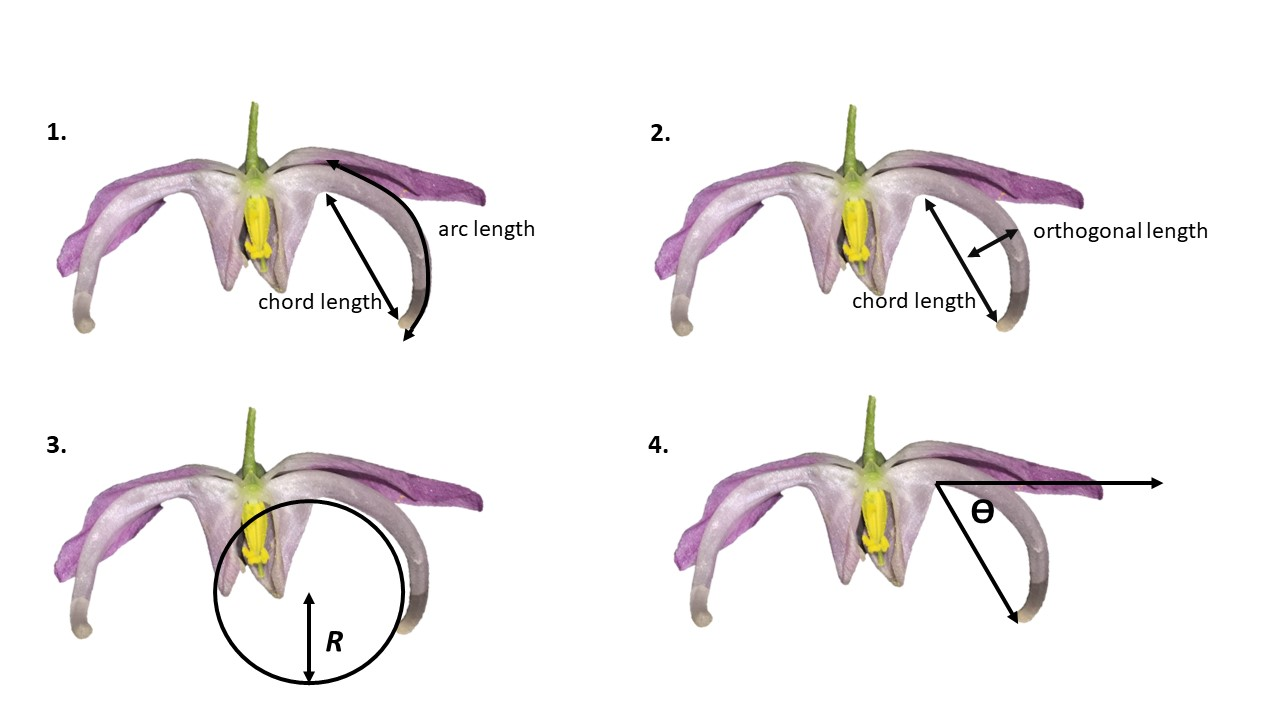
\includegraphics{Figures/Figure_1.jpg}
\caption{Figure 1. Overview of most commonly used curvature metrics. 1.
arc:chord ratio. 2. mandibular index 3. inverse radius. 4. angle of
deflection}
\end{figure}

Starting in 2010, geometric morphometrics (GM) emerges in the
pollination literature. GM comprises a set of protocols for quantifying
and comparing shapes. This approach has steadily gained in popularity
due to its mathematical rigour, reproducibility, and the appealing
visual representations of shape comparisons (\emph{e.g.} illustrations
of geographic variation in flower shape Gómez et al.
(\protect\hyperlink{ref-gomez_2009}{2009})). We briefly outline the
reasoning of a GM protocol to introduce relevant concepts, but recommend
the concise and authoritative introduction by Webster and Sheets
(\protect\hyperlink{ref-webster_2010}{2010}). A GM protocol for a 2-D
object begins by placing the specimens on an \emph{xy} grid and
assigning landmarks to locations on the specimen that are topologically
or biologically homologous. A landmark is defined so that its location
can be reproduced within and between samples. The set of landmarks
representing the shape of an organism is a `landmark configuration'. In
a comparative study, the samples are overlayed so that their shape
information is isolated from their orientation, location, and size. This
is done using a least-squares type protocol, most commonly the
Generalized Procrustes Analysis (GPA). GPA-adjusted landmark
configurations hereafter exist in a multidimensional shape space defined
by the number of landmarks and spatial dimensions implemented. Each
landmark configuration contains unique information about the specimen's
shape, and as such, occupies a unique position in the corresponding
shape space. These configurations are then ``projected'' onto a simpler
Euclidian space, similar to the reduction of a spherical Earth onto a
two-dimensional map (Webster and Sheets,
\protect\hyperlink{ref-webster_2010}{2010}). From here, familiar
statistical procedures (\emph{e.g.} PCA) can be performed to quantify
variation in landmark configurations (shape) between samples.

This is giant leap forward for morphological studies because GM is a
complete protocol for measuring, quantifying, and comparing shapes with
high precision, as well as the covariation of these shapes with
ecological variables of interest. Because GM has a traceable
mathematical lineage (Bookstein,
\protect\hyperlink{ref-bookstein_1997}{1997}), its vernacular is
well-defined and used consistently between practitioners. The limitation
of GM in quantifying curvature is that this method is concerned with
analyzing configurations of landmarks, \emph{i.e.} the entirety of a
shape summarized as a set of \emph{xy} coordinates. Once the specimen
has been reduced to a landmark configuration, it exists as a point in
shape space. Parsing segments of landmark configurations for separate
analyses (\emph{e.g.} for curvature) is not currently part of the
geometric morphometrics toolkit. Therefore, studies that have used this
technique to analyse biological forms are able to compare shapes in
their entirety, but are ultimately limited to making descriptive
statements about how segments of shapes appear to have different
curvatures (\emph{e.g.} Berns and Adams,
\protect\hyperlink{ref-berns_2013}{2013}).

Comment on Macleod 2002: Geometric morphometrics and geological
shape-classification systems

\begin{figure}
\centering
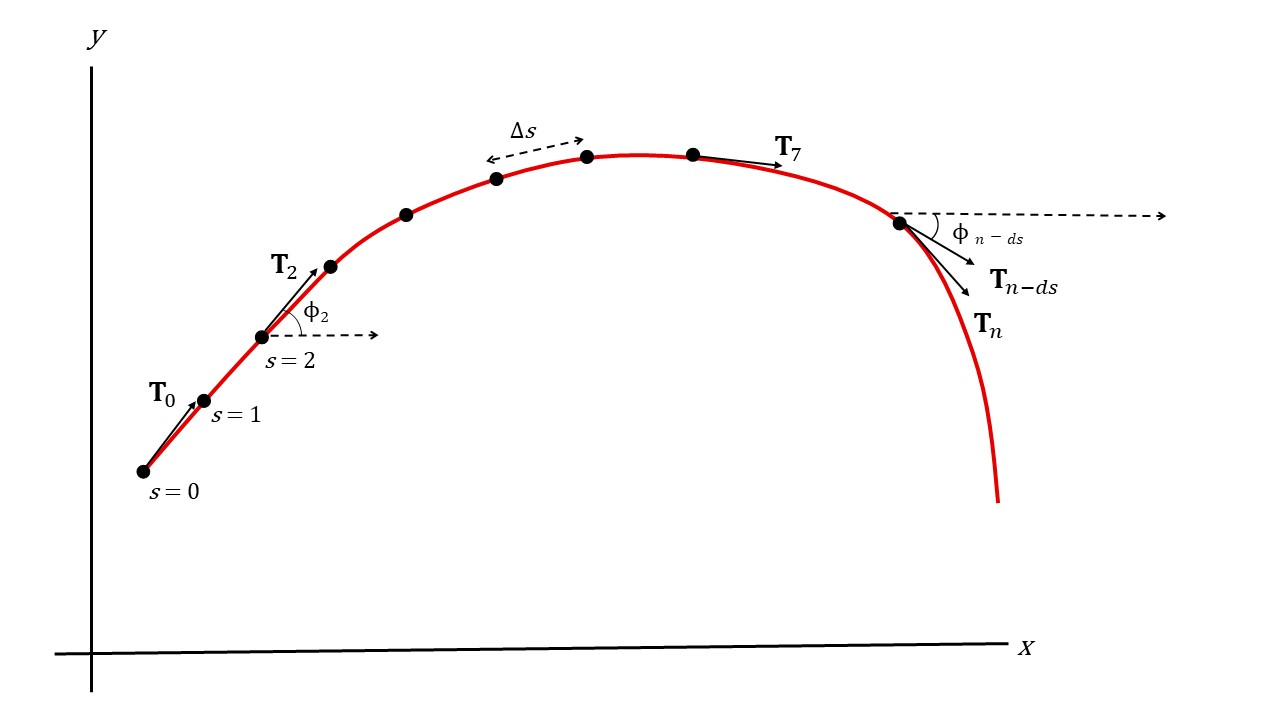
\includegraphics{Figures/Figure_2.jpg}
\caption{Figure 2. Overview of a geometric morphometrics protocol. 1.
Landmarks and semi-landmarks are assigned to a specimen. Each landmark
is assigned an \emph{xy} coordinate. 2. For each specimen a
configuration of landmarks exists as a single point in a non-Euclidian
shape space (abstracted here as a sphere segment). Red points represent
landmark configurations from other specimens. 3. Shape data is projected
onto a Euclidian plane -- a tangent space approximation. This allows
statistical analyses of shape variation (e.g.~principal components
analysis).}
\end{figure}

\hypertarget{what-is-curvature}{%
\paragraph{3. What is curvature?}\label{what-is-curvature}}

Reviewing the literature leads us to ask, ``what is curvature?''. Within
pollination ecology there are at least four metrics in use, with few
references to their origins or the the meaning of the associated units.
Therefore, we propose starting from first principles and turn to the
field of geometry. There, we again find several definitions resulting
from a history of independent derivations (reviewed in Coolidge,
\protect\hyperlink{ref-coolidge_1952}{1952}; Bardini and Gianella,
\protect\hyperlink{ref-bardini_2016}{2016}). Nonetheless these
definitions share a conceptual theme; curvature is a local property that
can measured point-wise on a line. This concept is fundamentally
different from those reviewed above where curvature is single property
of an entire shape. Here we follow the conventions of Casey
(\protect\hyperlink{ref-casey_1996}{1996}) and Rutter
(\protect\hyperlink{ref-rutter_2000}{2000}) and present a definition of
curvature that is tractable for analyzing biological shapes.

Intuitively, when a line deviates from being straight we say it is
curved, the extent to which it is not straight is its curvature. More
technically, a line deviates from being straight when its slope
(i.e.~the first derivative) changes direction - this is represented here
by the rotating tangent vectors \(\mathbf{T}_0\), \(\mathbf{T}_2\),
\(\mathbf{T}_8\), \(\mathbf{T}_n\) in \href{Figure_3.jpg}{Figure 3}.
Therefore, curvature can be thought of as the rate of change in the
tangent as we move across the curve. Hence, the tangents of a straight
line will have the same direction everywhere and a curvature of zero,
whereas the tangents of the curve shown in \href{Figure_3.jpg}{Figure 3}
will change direction and have a non-zero curvature.

To formalize these concepts mathematically we begin by considering an
ordinary function of the form \(y=f(x)\), where \(f(x)\) specifies one
value of \(y\) for each value of \(x\). Biological curves, however,
often loop back on themselves (e.g.~spirals) and are better described by
parametric fuctions that allow the curve to have multiple \(y\) values
for a single \(x\). Parametric functions use a `hidden' variable that
determines the values of \(x\) and \(y\) independently. Here, we use the
parameter variable arc length, \(s\), along the curve. We can then
express a position vector \(\mathbf{r}\) as a function solely of arc
length, \(s\). Specifically, using vector notation we have:

\$\$ \begin{equation}
\tag{1}

\mathbf{r}(s_i) =
\mathbf{r}_i \equiv \left[\begin{array}
{rrr}
x(s_i) \\
y(s_i) \\
\end{array}\right]

\end{equation} \$\$

Here \(\mathbf{r}_i\) is shorthand for \(\mathbf{r}(s_i)\) which
indicates that our position \((x(s_i), y(s_i))\) on the curve is
determined by the length of the segment \(s_i\). Although we could
parameterize a curve by many potential parametric variables, arc length
is a convienient choice because it allows us to move along the curve at
even increments, which we denote as \(\Delta s\). This proves useful
when taking repeated, equally-spaced measurements along a curve, such as
curvature.

As we are interested in the derivative properties of our arc-length
parameterized curve, we can differentiate \(\mathbf{r}(s)\) with respect
to arc length \(s\) in the following way (using the formal definition of
the derivative):

\$\$ \begin{equation}
\tag{2}

\lim\limits_{\Delta s \to 0} \frac{\Delta \mathbf{r}(s)}{\Delta s} = \frac{d \mathbf{r}(s)}{ds} = \mathbf{T}(s)  

\end{equation} \$\$

This produces a tangent function
\(\mathbf{T}(s) = \frac{d \mathbf{r}}{ds}\) giving the first derivative
of the parametric equation \(\mathbf{r}(s)\). The tangent
\(\mathbf{T}(s_i)\), represented by the shorthand \(\mathbf{T}_i\),
contains information about the direction of the curve at position
\(\mathbf{r}_i\) that we will use to calculate curvature.

At the beginning of this section we defined curvature, \(\kappa\), as
the rate at which the tangent is changing direction. We can now
formalize this by differentiating \(\mathbf{T}\) with respect to arc
length:

\$\$ \begin{equation}
\tag{3}

\kappa = \frac{d \mathbf{T}}{ds}

\end{equation} \$\$

Where \(\frac{d \mathbf{T}}{ds}\) is the second derivative of the
parameteric function \(\mathbf{r}(s_i)\):

\$\$ \begin{equation}
\tag{4}

\kappa_i = \lim\limits_{\Delta s \to 0} \frac{\mathbf{T}_i - \mathbf{T}_{i- \Delta s}}{\Delta s} = \frac{d \mathbf{T}_i}{ds}

\end{equation} \$\$

When the tangent \(\mathbf{T}\) is placed into a cartesian plane its
direction is related to the angle \(\phi\) formed with the \(x\)-axis
\href{Figures/Figure_3.jpg}{(Figure 3)}. Thus the \(x(s_i)\) and
\(y(s_i)\) components of the tangent vector \(\mathbf{T_i}\) can be
expressed as:

\$\$ \begin{equation}
\tag{5}

\mathbf{T_i} = 

\left[\begin{array}
{rrr}
x(s_i) \\
y(s_i) \\
\end{array}\right] =

\left[\begin{array}
{rrr}
cos(\phi_i) \\
sin(\phi_i) \\
\end{array}\right]

\end{equation} \$\$

Where:

\$\$ \begin{equation}
\tag{6}

\tan(\phi_i) = \frac{y(s_i)}{x(s_i)}

\end{equation} \$\$

And:

\$\$ \begin{equation}
\tag{7}

\phi_i = \arctan{\frac{y(s_i)}{x(s_i)}}

\end{equation} \$\$

Thus, curvature \(\kappa\) can be expressed as the change in the angle
\(\phi\) formed between the tangent \(\mathbf{T}\) and the \(x\)-axis:

\$\$ \begin{equation}
\tag{8}

\kappa = \frac{d \mathbf{T}}{ds} = \frac{d\phi}{ds}

\end{equation} \$\$

This definition provides an intuitive unit of measurement for reporting
curvature: degrees of rotation per unit arc length
\href{Figure_4.jpg}{(Figure 4)}. For example, if arc length has been
measured in millimeters, we would report its curvature as degrees per
millimeter \(degrees \cdot mm^{-1}\). Framed this way curvature is a
measure of rotation per distance. In contrast to previous defintions,
where curvature is an indivisble, single property of an entire shape,
here, curvature is a property of every point along the curve. Under our
point-wise defintion, we can summarize the \emph{total curvature}
(Milnor, \protect\hyperlink{ref-milnor_1954}{1954}) of a specimen as the
of sum the individual curvature measurements made along the curve:

\$\$ \begin{equation}
\tag{6}

\kappa_{total} = \int_{0}^{s_{max}} \kappa \; ds 

\end{equation} \$\$

Units for \emph{total curvature} are no longer expressed as
\(degrees \cdot mm^{-1}\) because we are not measuring curvature at a
single point. Instead we are summarizing all tangent rotations along the
curve, expressed simply as \(degrees\).

To account for size variation between specimens, we propose using
\emph{total adjusted curvature}, that is, total curvature divided by arc
length:

\$\$\begin{equation}
\tag{7}

\kappa_{adj} = \frac{\kappa_{total}}{s_{max}} 

\end{equation}\$\$

Units for \(\kappa_{adj}\) are expressed as \(degrees \cdot mm^{-1}\).
\emph{Total adjusted curvature} also represents mean curvature of the
curve.

\begin{figure}
\centering
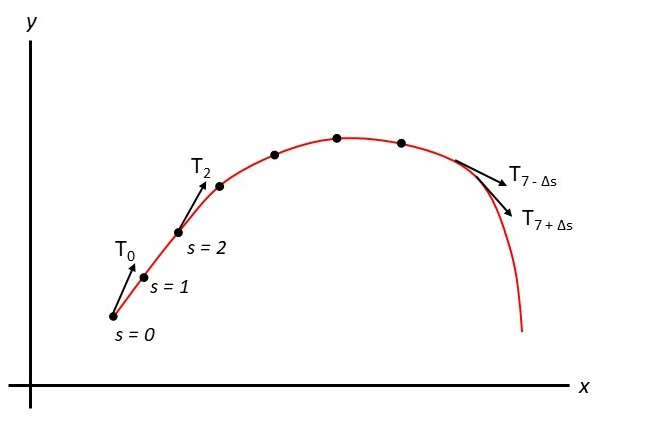
\includegraphics{Figures/Figure_3.jpg}
\caption{Figure 3. A curve parameterized by arc length, \(s\). When
\(s=8\), the vector \(\mathbf{r}(s_8)\) points to the location on the
curve \((x_8, y_8)\). \(T_0\), \(T_2\), and \(T_8\) are the tangents (
\(\frac{d \mathbf{r}}{ds}\) ) at \(s=0\), \(s=2\), and \(s=8\),
respectively. Curvature at \(s_i\) is defined in equation (4).}
\end{figure}

\hypertarget{a-proposed-protocol-for-measuring-curvature}{%
\paragraph{4. A proposed protocol for measuring
curvature}\label{a-proposed-protocol-for-measuring-curvature}}

As illustrated in the methodology review, our current protocols for
measuring flower-pollinator curvature lack a conceptual unity. There are
two main advantages of the curvature definition described above. First,
curvature becomes a local property of the tissue or organ under study.
This means that shape information is gathered at every point along the
curve and can be examined and compared to other points within or between
specimens. This differs from previous methods that take curvature as a
indivisible property of the entire specimen. Second, because the revised
definition is explicitly adapted from the field of differential
geometry, we benefit from established, well-defined concepts that make
clear what is meant by `curvature'. When the definition of curvature is
in agreement between these research areas, future advancements in
geometry can be more readily incorporated into morphological studies.

In order to apply this definition of curvature, a biological organ or
tissue needs to be reduced to a continuous function. To do this, we
propose a protocol as illustrated in \href{Figures/Figure_4.jpg}{Figure
4}. First, a specimen is landmarked at several locations along the area
of study (for landmark selection criteria see: Webster and Sheets
(\protect\hyperlink{ref-webster_2010}{2010})). Second, a mathematical
function is fitted to the landmarks. Finally, curvature is calculated
point-wise along the curve. Cosgrove
(\protect\hyperlink{ref-cosgrove_1990}{1990}) used an analogous approach
to study the development of cucumber hypocotyls. By fitting cubic
splines to images of seedlings, curvature was computed using the same
definition as above. However, since Cosgrove
(\protect\hyperlink{ref-cosgrove_1990}{1990}), the entire field of
landmark-based geometric morphometrics has unfolded (reviewed in Adams
et al., \protect\hyperlink{ref-adams_2013}{2013}). Whereas Cosgrove
(\protect\hyperlink{ref-cosgrove_1990}{1990}) marked images by hand,
landmark morphometrics incorporates digital imaging (including scaling)
to accurately mark homologous points between specimens. Using a similar
approach, Terral et al (\protect\hyperlink{ref-terral_2004}{2004})
employed digital landmarking of olive stones to estimate polynomial
equations that represented their shape (but did not calculate curvature
specifically). Synthesizing the concepts of Cosgrove
(\protect\hyperlink{ref-cosgrove_1990}{1990}) and Terral
(\protect\hyperlink{ref-terral_2004}{2004}) produces a modernized method
for fitting curves and computing curvature from biological forms
\href{Figures/Figure_4.jpg}{(Figure 4)}

\begin{figure}
\centering
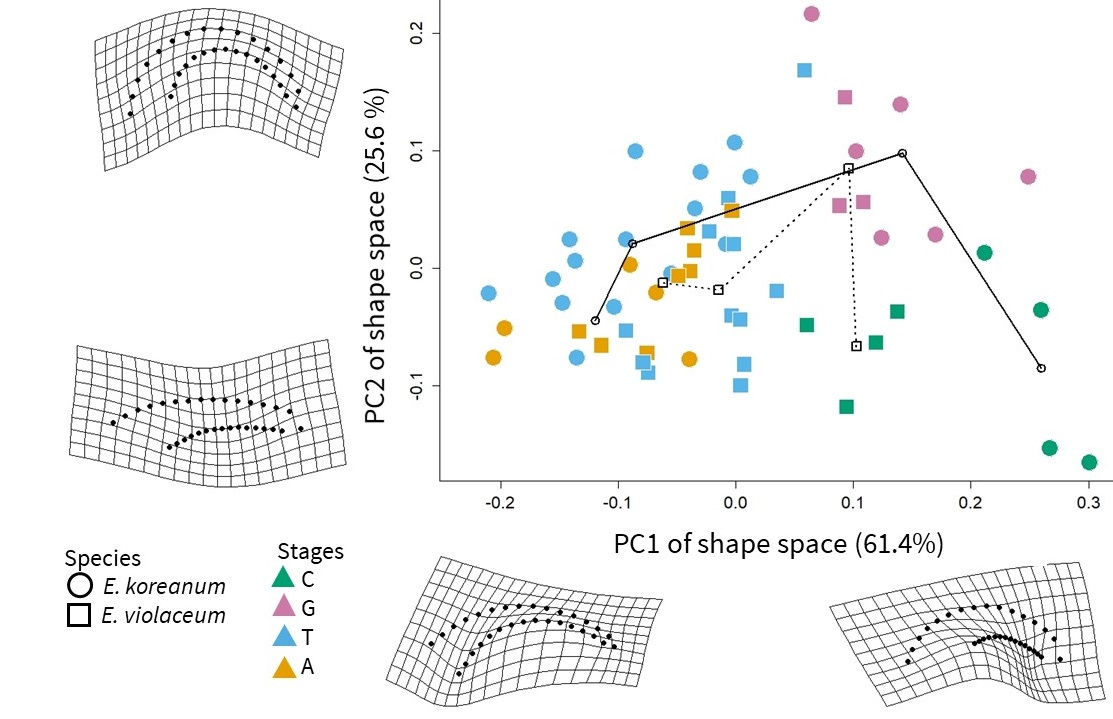
\includegraphics{Figures/Figure_4.jpg}
\caption{Figure 4: Proposed protocol for measuring curvature. 1. A petal
of \emph{Epimedium violaceum} is landmarked and rotated. 2. A polynomial
curve is fitted to the landmarks. 3. The tangent vector \(\mathbf{T}\)
is calculated at infinitesimal increments, \(ds\), along the curve. 4.
Curvature is calculated as the rate of change of the tangent vectors at
every point along the curve. Total curvature is calculated by the
methods outlined in Section 3.}
\end{figure}

Comment on why using we're using polynomials and not splines, fourier,
etc.

\hypertarget{proof-of-concept-a-study-of-the-development-of-curvature-in-epimedium}{%
\paragraph{\texorpdfstring{5. Proof of concept: A study of the
development of curvature in
\emph{Epimedium}}{5. Proof of concept: A study of the development of curvature in Epimedium}}\label{proof-of-concept-a-study-of-the-development-of-curvature-in-epimedium}}

We tested the utility of this curvature metric by studying floral
development in \emph{Epimedium grandiflorum} C.Morren, \emph{Epimedium
koreanum} Nakai, and \emph{Epimedium violaceum} C.Morren.
(Berberidaceae, Table S2). The latter two `species' are generally
considered forms of \emph{E. grandiflorum sensu lato} (Stearn,
\protect\hyperlink{ref-stearn_2002}{2002}), but we considered them
separate for comparitive purposes.

Flower size was measured daily from April 9 to May 2, 2019 at the UBC
Botanical Garden (Supp Mat 1). Size was defined as the length between
the apex of the two outer sepals lying on the major axis of the flower -
aestivation is imbricate. Length was measured to the nearest 0.1 mm
using an SPI Polymid Dial Caliper. By correlating changes in flower size
to developmental landmarks \href{Figures/Figure_5.jpeg}{(Figure 5)}, we
were able to define 3 discrete stages of flower development in \emph{E.
grandiflorum} and 4 stages in \emph{E. koreanum} and \emph{E. violaceum}
(Table S3, \& will include figure with photographs of the stages).

Flowering stage data was fragmented and staggered because of censoring,
i.e.~due to tracking flowers after their initial budding stage, or
flowers that had succumb to herbivory or weather after several days of
measurement. Therefore, stage data was aligned by using a multiple
sequence alignment protocol (ClustalW implemented in \texttt{msa} v.3.9)
with a neutral (identity) substitution matrix. Gap opening was
prohibited. By aligning phenological data within species, a consensus
(mean) stage sequence was calculated and used to estimate flower age
where observations were censored. Once aligned, these data represent the
`developmental dataset'.

To measure curvature, a separate set of \emph{Epimedium} flowers were
sampled haphazardly and preserved in 70\% ethanol. Preserved flowers
were later transferred to a glass slide and imaged in the lateral view
using a stereo microscope at 0.63x (Zeiss Stemi 508 with Axiocam 301).
Specimens that did not fit within the field of view were imaged in
halves and the images joined using the Stitching Plugin in the Fiji
distribution of ImageJ2 (Preibisch et al.,
\protect\hyperlink{ref-preibisch_2009}{2009}; Rueden et al.,
\protect\hyperlink{ref-rueden_2017}{2017}).

Photographed specimens were landmarked digitally using tpsDig (Rohlf,
\protect\hyperlink{ref-rohlf_2015}{2015}). We placed landmarks along the
edge of dorsal petals (in lateral view) as an approximation of the
flowers' total shape (see discussion of geometric morphometrics above).
Landmarks used to measure the dorsal arc were 1) the farthest point on
the apex of the spur before the inflection point where either the spur
diminishes to a tip (\emph{E. violaceum}) or widens into a saccate
reservoir (\emph{E. koreanum}), and 2) the inflection point at which the
spur widens to become an attachment for the petal to the stem
(anatomical name?). 13 semi-landmarks (defined in Webster and Sheets,
\protect\hyperlink{ref-webster_2010}{2010}) were placed between
landmarks 1 and 2 (illustrated in \href{Figures/Figure_S2.jpg}{Figure
S2}.

Landmark files (.tps) were imported into R using \texttt{Momocs} v.1.3.0
(Bonhomme et al., \protect\hyperlink{ref-bonhomme_2014}{2014}).
Polynomial functions were regressed to the landmark coordinates for each
specimen using \texttt{Momocs} - we chose polynomials of the third
degree based on the recommendations of Rolhf
(\protect\hyperlink{ref-rohlf_1990}{1990}). Arc length was calculated
from bounded polynomial functions using \texttt{pracma} v.2.2.5
(Borchers, \protect\hyperlink{ref-borchers_2019}{2019}). Curvature, as
defined in the previous section, was computed using custom functions
modified from the \texttt{maxcurv()} function of the
\texttt{soilphysics} package v.3.1 (Silva and Lima,
\protect\hyperlink{ref-silva_2017}{2017}). All custom functions used in
this analysis are available as an R package \texttt{curvy} hosted at
github.com/mannfred/curvy. R scripts used in this analysis are hosted at
github.com/mannfred/epidmedium. These data represent the `curvature
dataset'.

Results:

In \emph{E. grandiflorum} we identified three distinct stages of
development (Table S3). The first stage (``G'') is defined as the
initiation and growth of the bud until the petals begin to separate
(``T'' stage). At the ``T'' stage nectar begins accumilating in the
spurs. Anthesis takes place during the ``A'' stage at which point the
flower opening may increase in size and anthers dehisce. In \emph{E.
koreanum} and \emph{E. violaceum} we detected another distinct ``C''
stage in the early stage of bud development. At this stage the petals
are shorter in length than the sepals that envelop them - the ``G''
stage begins when the petals overtake the surrounding sepals in length.

\begin{figure}
\centering
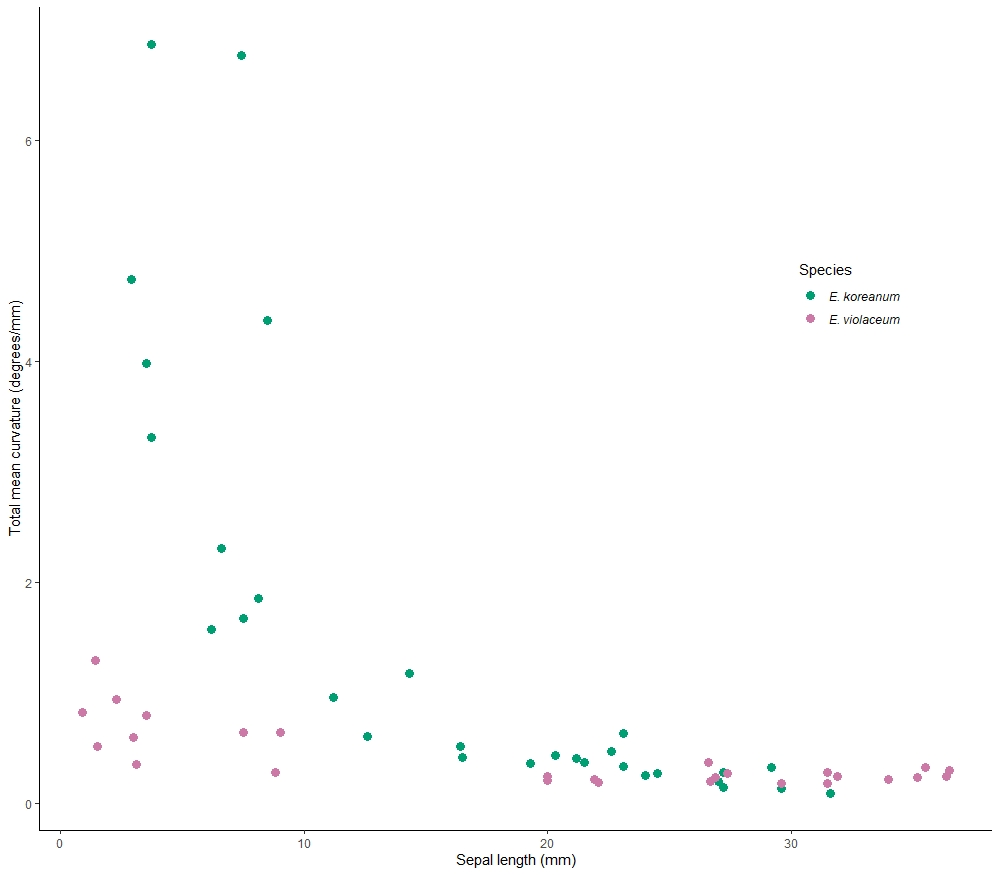
\includegraphics{Figures/Figure_5.jpeg}
\caption{Figure 5: Comparison of developmental stages. Size is in mm.
Tukey's HSD: p\textless{}0.01 for all within-species comparisons}
\end{figure}

We found that \emph{E. koreanum} is more curved at initial stages of
development, but curvature is similar once sepal size exceeds 20mm:

\begin{figure}
\centering
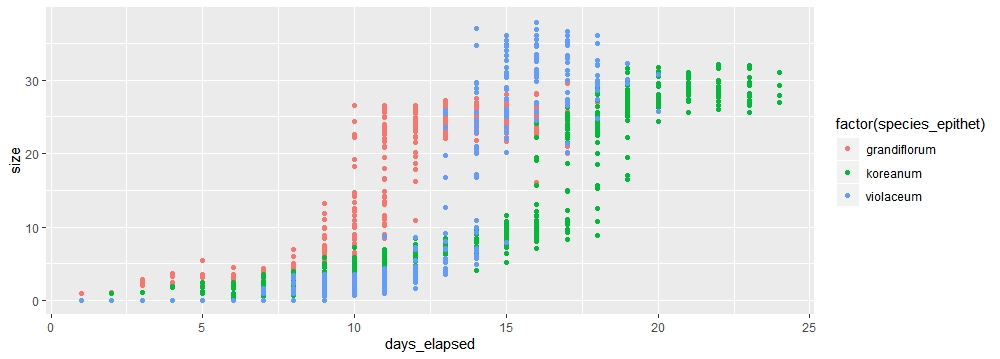
\includegraphics{Figures/Figure_6.jpeg}
\caption{Figure 6: size vs curvature}
\end{figure}

\begin{longtable}[]{@{}lll@{}}
\caption{Table 1: Summary of literature reviewed for the role of
curvature in plant-pollinator systems.}\tabularnewline
\toprule
Citation & System & Stated.Method..Inferred.Method.\tabularnewline
\midrule
\endfirsthead
\toprule
Citation & System & Stated.Method..Inferred.Method.\tabularnewline
\midrule
\endhead
feinsinger\_1978 & Community organization among neotropical
nectar-feeding birds & arc:chord ratio\tabularnewline
snow\_1972 & Feeding niches of hummingbirds in a Trinidad valley &
qualitative\tabularnewline
stiles\_1975 & Corolla morphology of Heliconia and bill morphology of
nine hummingbird species at La Selva, Costa Rica. & Qualitative
(e.g.~`strongly curved, moderately curved, etc.).\tabularnewline
buttrose\_1977 & Significance of curvature of style branches in Hibiscus
trionum for pollination & Qualitative\tabularnewline
gill\_1978 & Sunbird bill diversity and abilities to extract nectar from
Kenyan Leonotis nepetifolia (Lamiaceae). & Not defined (Mandibular
index): Curvature is ``the ratio x/y, where x is the bill length
measured from the anterior edge of the nostril and y is the maximum
height above the longest chord of the bill.''\tabularnewline
carothers\_1982 & Effects of Trophic Morphology and Behavior on Foraging
Rates of Three Hawaiian Honeycreeper & Not defined (angle of
deflection): based on use of degrees to express curvature\tabularnewline
grant\_1983 & Hawkmoth pollination of Mirabilis longiflora
(Nyctaginaceae) & qualitative\tabularnewline
paton\_1989 & Correlates (Geography, Age, Sex, Tongue structure,
foraging mode) of bill morphology on nectar extraction 198 hummers (and
other birds). & Curvature index (Mandibular index): ``Bill curvatures
were defined as the maximum perpendicular height of the bottom edge of
the culmen above the chord from the gape to the tip of the bill, divided
by the length of this chord''.\tabularnewline
muller\_1995 & curved bristles on the proboscis on European bees for the
extraction of pollen. & qualitative\tabularnewline
smith\_1995 & Evolutionary Consequences of Extinctions in Populations of
a Hawaiian Honeycreepe & inverse radius\tabularnewline
stiles\_1995 & Effects of bill morphology on insect foraging strategy by
11 species of hummingbirds at La Selva, Costa Rica. & Arc:chord ratio of
exposed culmen -- silhouette projected onto a screen.\tabularnewline
mcintyre\_1996 & Phototropism in Helianthus and effects on cotyledon
curvature & Protractor - further details not provided, presumably angle
of deflection method.\tabularnewline
manning\_1997 & Tangle-veined fly pollination of South African
Iridaceace, Geraniaceae, Orchidaceae & qualitative\tabularnewline
cotton\_1998 & Survey and description of 16 hummingbird species
occurring at Amacayacu National Park, Colombia. &
Qualitative\tabularnewline
oritz\_2000 & Pollination and breeding system of Putoria calabrica
(Rubiaceae), a Mediterranean dwarf shrub & qualitative\tabularnewline
temeles\_2000 & Sexual dimorphism of bill shape in Purple-throated
caribs (Eulampis jugularis), pollinatiors of Heliconia at Quilesse
Reserve, Saint Lucia. & Not described, but presumably the same method as
Temeles 2009, Temeles 2010.\tabularnewline
borgella\_2001 & Effects of bill morphology (21 hummingbird spp.) on
pollen loads (35 plant spp.) at Coto Brus, Costa Rica. & Not defined:
``For species with decurved bills, we also used a ruler to measure a few
bills along the curve to calculate a correction factor.''\tabularnewline
temeles\_2003 & Floral curvature in Heliconia pollinated by
Purple-throated caribs (Eulampis jugularis) & Not described, but
presumably the same method as Temeles 2010, Temeles 2009.\tabularnewline
travers\_2003 & Nectar spurs of Impatiens spp. and Ruby-throated
hummingbird (Archilochus colubris) at Franklin County, Massachusetts. &
``Angle at which the spur deviates from an arbitrary line drawn through
the flower.'' (Angle of deflection)\tabularnewline
temeles\_2005 & Sexual dimorphism of bill shape in Purple-throated
caribs (Eulampis jugularis), pollinatiors of Heliconia at Quilesse
Reserve, Saint Lucia. & Not described, but presumably the same method as
Temeles 2010, Temeles 2009.\tabularnewline
collins\_2008 & Foraging efficiency from artificial and natural (15
spp.) flowers by 4 species of hummingbirds at Monteverde, Costa Rica &
Paton and Collins 1989\tabularnewline
stiles\_2008 & Correlations of bill morphology to the elevational
distributions of 150 spp. of hummingbirds in the Andes. & Arc:chord
ratio of exposed culmen\tabularnewline
young\_2008 & Selection on spur shape in Impatiens capensis &
travers\_2003\tabularnewline
marten\_2009 & Testing the pollination syndrome hypothesis in Antillean
Gesneriaceae. & Protractor aligned with the dorsal side of the corolla
tube. (Angle of deflection)\tabularnewline
temeles\_2009 & Effects of natural (Heliconia) and artificial flower
morphologies on foraging performance of Purple-throated caribs (Eulampis
jugularis) at Saint Lucia. & Inverse radius calculated from the angle of
declension method.\tabularnewline
luo\_2010 & Effects of light and low temperature on the reciprocal style
curvature of Flexistylous Alpinia Species (Zingiberaceae) & angle of
deflection\tabularnewline
temeles\_2010 & Sexual dimorphism of bill shape in 21 species of Central
and South American hummingbirds. & Inverse radius calculated from the
angle of declension method.\tabularnewline
berns\_2010 & Sexual dimorphism of bill shape in Black-chinned
hummingbird (Archilochus alexandri) and Ruby-throated hummingbird
(Archilochus colubris). & Comparison of 3 methods: Paton and Collins
1989 (maxilla), Stiles 1975 (mandible), Temeles 2009 (inverse
radius).\tabularnewline
berns\_2013 & Sexual dimorphism of bill shape in 219 hummingbird spp. &
Geometric morphometrics ('' Thin-plate spline deformation grids revealed
that in these species, females have longer, more curved bills at both
the tip and main body of the bill relative to the mean, while males have
straighter and shorter bills and M. minima has the largest magnitude of
sexual shape dimorphism'' -- used GeoMorphometrics but in the end resort
to just saying that the deformations of the spline `look
different'.)\tabularnewline
wang\_2013 & Pollinators and nectar robbers cause directional selection
for large spur circle in Impatiens oxyanthera (Balsaminaceae) & angle of
deflection\tabularnewline
maglianesi\_2014 & Trait matching and resource use in a
plant-hummingbird network, La Selva, Costa Rica. & Angle of
deflection\tabularnewline
rico\_2014 & Bills as weapons in lekking Phaethornis longirostris at La
Selva, Costa Rica. & Arc:chord ratio of exposed culmen.\tabularnewline
alexandre\_2015 & QTL analysis comparing hummingbird pollinated and
generalist Rhytidophyllum flowers (Gesneriaceae). & Angle between flower
opening and flower base.\tabularnewline
campos\_2015 & Generating 3D printed flowers to test efficacy of moth
pollination & ``Curvature parameter''\tabularnewline
maglianesi\_2015\_a & Differential preferences of artificial and natural
(65 spp.) flower populations visited by 3 species of hummingbird in
Braulio Carrillo National Park, Costa Rica. & Angle of
deflection\tabularnewline
maglianesi\_2015\_b & Plant-pollinator specialization along an
elevational gradient at Braulio Carrillo National Park, Costa Rica. 21
hummingbird spp. and 208 plant species examined. & Angle of
deflection\tabularnewline
rocha\_2015 & Auxin and physical constraint exerted by the perianth
promote androgynophore bending in Passiflora mucronata L.
(Passifloraceae) & Not defined, inferred to be arc:chord ratio from
Methods\tabularnewline
miller\_2017 & Ecological Divergence among Closely Related,
Morphologically Similar Honeyeaters (Aves: Meliphagidae) Co-occurring in
Arid Australian Environments & arch:chord ratio\tabularnewline
lagomarsino\_2017 & Evolution of pollination syndromes in Andean
Campanulaceae. & Arc:chord ratio of corolla midline and base-to-opening
line.\tabularnewline
boehm\_2018 & Review of nectar robbing in Centropogon &
qualitative\tabularnewline
hadley\_2018 & Effects of forest fragmentation on hummingbird bill
morphologies (19 spp.) representative of specialization. Coto Brus,
Costa Rica. & Bill curvature was calculated as the angle between a
horizontal line across the top of the bill and a line running the length
of the bill. (Arc:chord ratio)\tabularnewline
partida\_2018 & Spatio?temporal structure of the taxonomic and
functional diversity of hummingbirds at the biosphere reserve El
Triunfo, Chiapas, Mexico & Inverse radius method, cites
temeles\_2009\tabularnewline
peng\_2019 & Morphospace exploration reveals divergent fitness optima
between plants and pollinators & same as campos\_2015: note that the c
parameter in our equation is not equivalent to the definition of
curvature in mathematics\tabularnewline
sonne\_2019 & Distribution of morphological specialization along an
elevational gradientin Ecuador. & Arc:chord ratio of exposed culmen and
corolla tubes\tabularnewline
\bottomrule
\end{longtable}

\begin{longtable}[]{@{}lll@{}}
\caption{Table S1: Additional literature reviewed for the role of
curvature in plant-pollinator systems.}\tabularnewline
\toprule
Citation & System & Method\tabularnewline
\midrule
\endfirsthead
\toprule
Citation & System & Method\tabularnewline
\midrule
\endhead
baldwin\_1931 & Measurements of birds & Inverse radius
method\tabularnewline
hamilton\_1975 & Comparative Behavior of the American Avocet and the
Black-Necked Stilt(Recurvirostridae) & Radius of
curvature\tabularnewline
mountainspring\_1987 & sexual dimorphism and foraging preferences of the
Hawaiian honeycreeper (Pseudonestor xanthophrys) & mandibular
index\tabularnewline
lindqvist\_2003 & Cladogenesis and reticulation in the Hawaiianendemic
mints (Lamiaceae) & qualitative\tabularnewline
ruan\_2008 & The impact of pollen tube growth on stigma lobe curvature
in Kosteletzkya virginica: the best of both worlds &
qualitative\tabularnewline
kawabata\_2009 & Quantitative analysis of corolla shapes and petal
contours in single-flower cultivars of Lisianthus. & Something like
geomorph??\tabularnewline
dalayap\_2011 & Petal, sepal, and labellum shapes in Mokara orchids &
Outline morphometrics\tabularnewline
nii\_2011 & Assessment of the Association between the Three-dimensional
Shape of the Corolla and Two-dimensional Shapes of Petals Using Fourier
Descriptors and Principal Component Analysis in Eustoma grandiflorum &
Fourier Transform, but lacks units for curvature K\tabularnewline
berger\_2017 & Quantifying morphological modifications to floral form in
gene knockdowns in Fedia graciliflora. & Landmark-based geometric
morphometrics\tabularnewline
dellinger\_2018 & Floral trait changes correlated with the repeated
shifts away from buzz?pollination in the Melastomataceae. &
Qualitative\tabularnewline
joly\_2018 & Analysis of polliation syndromes in Antillean Gesneriaceae.
& Geometric morphometrics. ``PC2 represents variation in corolla
curvature'' (descriptive).\tabularnewline
pour\_2018 & Curvature-based pattern recognition for cultivar
classification of Anthurium (Araceae) flowers. & Calculated k (the rate
of change in the direction of the tangent line at that point with
respect to arc length) for n points along the flower.\tabularnewline
song\_2018 & Quantitative Classification of the Morphological Traits of
Ray Florets in Large-flowered Chrysanthemum & angle of
declension\tabularnewline
\bottomrule
\end{longtable}

\begin{longtable}[]{@{}ll@{}}
\caption{Table S1: Sample sizes.}\tabularnewline
\toprule
Species & sample\_size\tabularnewline
\midrule
\endfirsthead
\toprule
Species & sample\_size\tabularnewline
\midrule
\endhead
\bottomrule
\end{longtable}

\begin{longtable}[]{@{}lllrrrrl@{}}
\caption{Table S3: Stages of \emph{Epimedium} flower
development.}\tabularnewline
\toprule
Stage & Defintion & Species\_epithet & mean\_size\_mm & loCI & hiCI &
stdv & elapsed\_days\tabularnewline
\midrule
\endfirsthead
\toprule
Stage & Defintion & Species\_epithet & mean\_size\_mm & loCI & hiCI &
stdv & elapsed\_days\tabularnewline
\midrule
\endhead
C & Petals do not exceed the length of the inner and outer sepals. &
koreanum & 3.257576 & 2.928715 & 3.586436 & 0.1665509 & 8.31 +/- 0.40
days\tabularnewline
& & violaceum & 1.351376 & 1.134264 & 1.568488 & 0.1095322 & 8.27 +/-
0.40 days\tabularnewline
G & Petals exceed the length of the inner and outer sepals. &
grandiflorum & 4.360494 & 3.779331 & 4.941657 & 0.2920325 & 7.01 +/-
0.45 days\tabularnewline
& & koreanum & 8.075000 & 7.774979 & 8.375021 & 0.1514640 & 14.3 +/-
0.20 days\tabularnewline
& & violaceum & 4.202128 & 3.648398 & 4.755858 & 0.2750913 & 12.0 +/-
0.20 days\tabularnewline
T & Opening and separation of the petals. At least one petal is free
from touching adjacent petals. Outer sepals begin to abscise. Nectar is
visibly collecting in spurs. & grandiflorum & 17.050909 & 15.689253 &
18.412565 & 0.6870223 & 10.9 +/- 0.20 days\tabularnewline
& & koreanum & 18.157143 & 16.881331 & 19.432954 & 0.6421844 & 17.1 +/-
0.20 days\tabularnewline
& & violaceum & 20.657895 & 18.317896 & 22.997894 & 1.1681067 & 14.1 +/-
0.20 days\tabularnewline
A & Initiated by partial anther dehiscence, followed by complete
dehiscence, and finally flower abscisson & grandiflorum & 24.627778 &
24.384224 & 24.871331 & 0.1235008 & 14.7 +/- 0.20 days\tabularnewline
& & koreanum & 27.794152 & 27.485873 & 28.102431 & 0.1561682 & 20.6 +/-
0.30 days\tabularnewline
& & violaceum & 31.560000 & 30.872686 & 32.247314 & 0.3472547 & 16.7 +/-
0.30 days\tabularnewline
\bottomrule
\end{longtable}

\begin{figure}
\centering
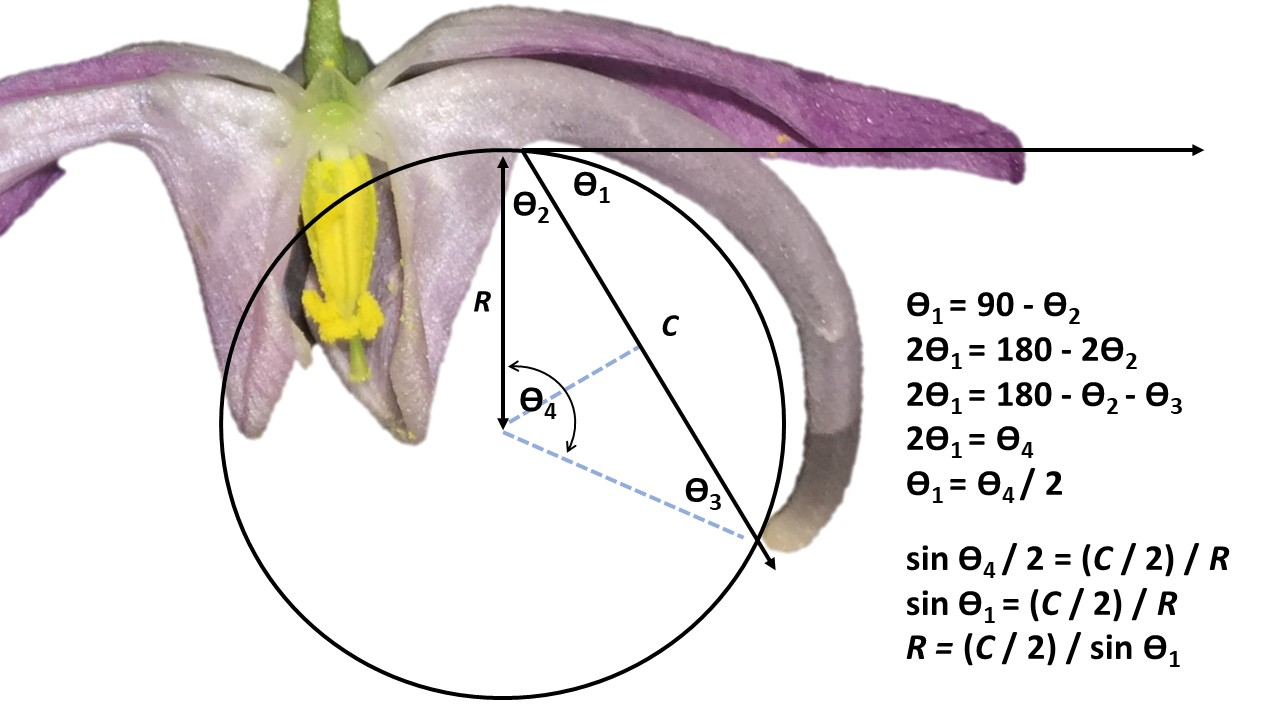
\includegraphics{Figures/Figure_S1.jpg}
\caption{Figure S1. Demonstration that the angle of deflection and
inverse radius methods are interchangeable}
\end{figure}

\begin{figure}
\centering
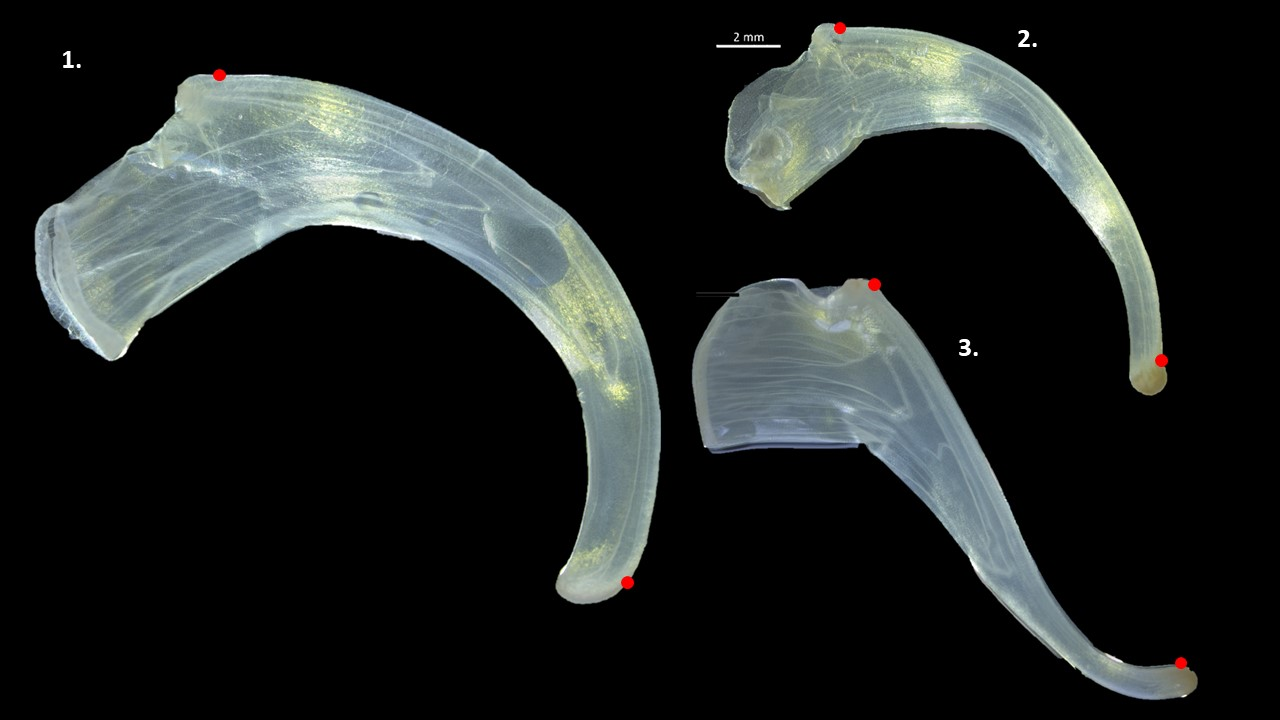
\includegraphics{Figures/Figure_S2.jpg}
\caption{Figure S2. Landmarking \emph{Epimedium} specimens. Left:
\emph{E. koreanum}, Top Right: \emph{E. violaceum}, Bottom Right:
\emph{E. grandiflorum}.}
\end{figure}

\begin{figure}
\centering
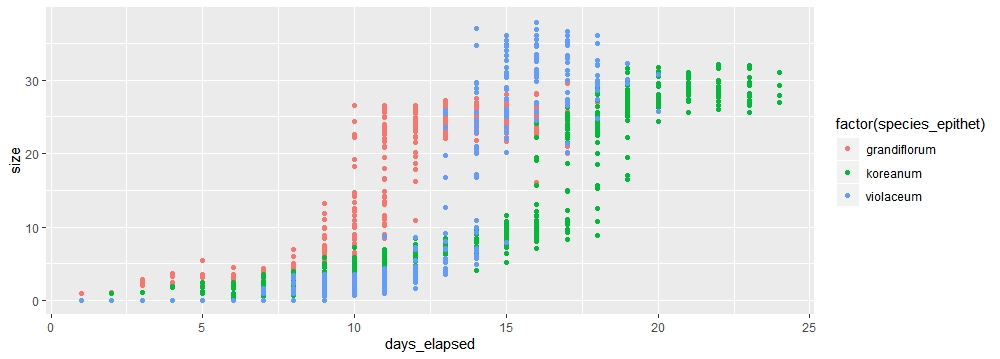
\includegraphics{Figures/Figure_S3.jpeg}
\caption{Figure S3. Logistic growth of Epimedium flowers}
\end{figure}

\hypertarget{references}{%
\section{References}\label{references}}

\setlength{\parindent}{-0.2in}
\setlength{\leftskip}{0.2in}
\setlength{\parskip}{8pt}

\noindent

\hypertarget{refs}{}
\leavevmode\hypertarget{ref-adams_2013}{}%
Adams, D.C., Rohlf, F.J., and Slice, D.E. (2013). A field comes of age:
Geometric morphometrics in the 21st century. Hystrix \emph{24}, 7.

\leavevmode\hypertarget{ref-armbruster_2009}{}%
Armbruster, W.S., and Muchhala, N. (2009). Associations between floral
specialization and species diversity: Cause, effect, or correlation?
Evolutionary Ecology \emph{23}, 159.

\leavevmode\hypertarget{ref-baldwin_1931}{}%
Baldwin, S.P., Oberholser, H.C., and Worley, L.G. (1931). Measurements
of birds (Cleveland Museum of Natural History).

\leavevmode\hypertarget{ref-bardini_2016}{}%
Bardini, G., and Gianella, G.M. (2016). A historical walk along the idea
of curvature, from Newton to Gauss passing from Euler. International
Mathematical Forum \emph{11}, 259--278.

\leavevmode\hypertarget{ref-bell_1956}{}%
Bell, J. (1956). 2619. Tangent, chord theorem. The Mathematical Gazette
\emph{40}, 211--212.

\leavevmode\hypertarget{ref-berns_2010}{}%
Berns, C.M., and Adams, D.C. (2010). Bill shape and sexual shape
dimorphism between two species of temperate hummingbirds: Black-Chinned
hummingbird (\emph{Archilochus alexandri}) and Ruby-Throated hummingbird
(\emph{Archilochus colubris}). The Auk \emph{127}, 626--635.

\leavevmode\hypertarget{ref-berns_2013}{}%
Berns, C.M., and Adams, D.C. (2013). Becoming different but staying
alike: Patterns of sexual size and shape dimorphism in bills of
hummingbirds. Evolutionary Biology \emph{40}, 246--260.

\leavevmode\hypertarget{ref-bluthgen_2006}{}%
Blüthgen, N., Menzel, F., and Blüthgen, N. (2006). Measuring
specialization in species interaction networks. BMC Ecology \emph{6}, 9.

\leavevmode\hypertarget{ref-bonhomme_2014}{}%
Bonhomme, V., Picq, S., Gaucherel, C., and Claude, J. (2014). Momocs:
Outline analysis using r. Journal of Statistical Software \emph{56},
1--24.

\leavevmode\hypertarget{ref-bookstein_1997}{}%
Bookstein, F.L. (1997). Morphometric tools for landmark data: Geometry
and biology (Cambridge University Press).

\leavevmode\hypertarget{ref-borchers_2019}{}%
Borchers, H.W. (2019). Pracma: Practical numerical math functions. R
package version 2.2.5.

\leavevmode\hypertarget{ref-cardinal_2013}{}%
Cardinal, S., and Danforth, B.N. (2013). Bees diversified in the age of
eudicots. Proceedings of the Royal Society B: Biological Sciences
\emph{280}, 20122686.

\leavevmode\hypertarget{ref-carothers_1982}{}%
Carothers, J.H. (1982). Effects of trophic morphology and behavior on
foraging rates of three hawaiian honeycreepers. Oecologia \emph{55},
157--159.

\leavevmode\hypertarget{ref-casey_1996}{}%
Casey, J. (1996). Exploring curvature (Braunschweig, Germany: Friedr.
Vieweg \& Sohn Verlagsgesellschaft mbH).

\leavevmode\hypertarget{ref-coen_2016}{}%
Coen, E., and Rebocho, A.B. (2016). Resolving conflicts: Modeling
genetic control of plant morphogenesis. Developmental Cell \emph{38},
579--583.

\leavevmode\hypertarget{ref-collins_2008}{}%
Collins, B.G. (2008). Nectar intake and foraging efficiency: Responses
of honeyeaters and hummingbirds to variations in floral environments.
The Auk \emph{125}, 574--587.

\leavevmode\hypertarget{ref-coolidge_1952}{}%
Coolidge, J.L. (1952). The unsatisfactory story of curvature. The
American Mathematical Monthly \emph{59}, 375--379.

\leavevmode\hypertarget{ref-cosgrove_1990}{}%
Cosgrove, D.J. (1990). Rapid, bilateral changes in growth rate and
curvature during gravitropism of cucumber hypocotyls: Implications for
mechanism of growth control. Plant, Cell \& Environment \emph{13},
227--234.

\leavevmode\hypertarget{ref-dehling_2014}{}%
Dehling, D.M., Töpfer, T., Schaefer, H.M., Jordano, P., Böhning-Gaese,
K., and Schleuning, M. (2014). Functional relationships beyond species
richness patterns: Trait matching in plant--bird mutualisms across
scales. Global Ecology and Biogeography \emph{23}, 1085--1093.

\leavevmode\hypertarget{ref-feinsinger_1978}{}%
Feinsinger, P., and Colwell, R.K. (1978). Community organization among
neotropical nectar-feeding birds. American Zoologist \emph{18},
779--795.

\leavevmode\hypertarget{ref-gomez_2009}{}%
Gómez, J., Perfectti, F., Bosch, J., and Camacho, J. (2009). A
geographic selection mosaic in a generalized
plant--pollinator--herbivore system. Ecological Monographs \emph{79},
245--263.

\leavevmode\hypertarget{ref-graham_2009}{}%
Graham, C.H., Parra, J.L., Rahbek, C., and McGuire, J.A. (2009).
Phylogenetic structure in tropical hummingbird communities. Proceedings
of the National Academy of Sciences \emph{106}, 19673--19678.

\leavevmode\hypertarget{ref-grant_1949}{}%
Grant, V. (1949). Pollination systems as isolating mechanisms in
angiosperms. Evolution \emph{3}, 82--97.

\leavevmode\hypertarget{ref-hainsworth_1973}{}%
Hainsworth, F.R. (1973). On the tongue of a hummingbird: Its role in the
rate and energetics of feeding. Comparative Biochemistry and Physiology
Part A: Physiology \emph{46}, 65--78.

\leavevmode\hypertarget{ref-kay_2009}{}%
Kay, K.M., and Sargent, R.D. (2009). The role of animal pollination in
plant speciation: Integrating ecology, geography, and genetics. Annual
Review of Ecology, Evolution, and Systematics \emph{40}, 637--656.

\leavevmode\hypertarget{ref-lagomarsino_2019}{}%
Lagomarsino, L.P., and Muchhala, N. (2019). A gradient of pollination
specialization in three species of bolivian centropogon. American
Journal of Botany \emph{106}, 633--642.

\leavevmode\hypertarget{ref-maglianesi_2014}{}%
Maglianesi, M.A., Blüthgen, N., Böhning-Gaese, K., and Schleuning, M.
(2014). Morphological traits determine specialization and resource use
in plant--hummingbird networks in the neotropics. Ecology \emph{95},
3325--3334.

\leavevmode\hypertarget{ref-maglianesi_2015_b}{}%
Maglianesi, M.A., Blüthgen, N., Böhning-Gaese, K., and Schleuning, M.
(2015). Functional structure and specialization in three tropical
plant--hummingbird interaction networks across an elevational gradient
in costa rica. Ecography \emph{38}, 1119--1128.

\leavevmode\hypertarget{ref-milnor_1954}{}%
Milnor, J. (1954). On total curvatures of closed space curves.
Mathematica Scandinavica \emph{1}, 289--296.

\leavevmode\hypertarget{ref-minnaar_2019}{}%
Minnaar, C., Jager, M. de, and Anderson, B. (2019). Intraspecific
divergence in floral-tube length promotes asymmetric pollen movement and
reproductive isolation. New Phytologist.

\leavevmode\hypertarget{ref-nath_2003}{}%
Nath, U., Crawford, B.C., Carpenter, R., and Coen, E. (2003). Genetic
control of surface curvature. Science \emph{299}, 1404--1407.

\leavevmode\hypertarget{ref-vanderniet_2012}{}%
Niet, T. van der, and Johnson, S.D. (2012). Phylogenetic evidence for
pollinator-driven diversification of angiosperms. Trends in Ecology \&
Evolution \emph{27}, 353--361.

\leavevmode\hypertarget{ref-ollerton_2017}{}%
Ollerton, J. (2017). Pollinator diversity: Distribution, ecological
function, and conservation. Annual Review of Ecology, Evolution, and
Systematics \emph{48}, 353--376.

\leavevmode\hypertarget{ref-preibisch_2009}{}%
Preibisch, S., Saalfeld, S., and Tomancak, P. (2009). Globally optimal
stitching of tiled 3D microscopic image acquisitions. Bioinformatics
\emph{25}, 1463--1465.

\leavevmode\hypertarget{ref-robertson_1889}{}%
Robertson, C. (1889). Flowers and insects. II. Botanical Gazette
\emph{14}, 172--178.

\leavevmode\hypertarget{ref-rohlf_2015}{}%
Rohlf, F.J. (2015). The tps series of software. Hystrix \emph{26}.

\leavevmode\hypertarget{ref-rohlf_1990}{}%
Rolhf, F.J. (1990). Fitting curves to outlines. In Proceedings of the
Michigan Morphometrics Workshop, F.J. Rolhf, and F.L. Bookstein, eds.
(Ann Arbor, MI: University of Michigan Museum of Zoology), pp. 177--188.

\leavevmode\hypertarget{ref-rueden_2017}{}%
Rueden, C.T., Schindelin, J., Hiner, M.C., DeZonia, B.E., Walter, A.E.,
Arena, E.T., and Eliceiri, K.W. (2017). ImageJ2: ImageJ for the next
generation of scientific image data. BMC Bioinformatics \emph{18}, 529.

\leavevmode\hypertarget{ref-rutter_2000}{}%
Rutter, J.W. (2000). Geometry of curves (Boca Raton, FL: CRC Press,
Taylor; Francis Group).

\leavevmode\hypertarget{ref-scott-elliot_1890}{}%
Scott-Elliot, G. (1890). Ornithophilous flowers in south africa. Annals
of Botany \emph{4}, 265--280.

\leavevmode\hypertarget{ref-silva_2017}{}%
Silva, A.R. da, and Lima, R.P. de (2017). Determination of maximum
curvature point with the r package soilphysics. International Journal of
Current Research \emph{9}, 45241--45245.

\leavevmode\hypertarget{ref-sonne_2019}{}%
Sonne, J., Zanata, T.B., Martı́n González, A.M., Cumbicus Torres, N.L.,
Fjeldså, J., Colwell, R.K., Tinoco, B.A., Rahbek, C., and Dalsgaard, B.
(2019). The distributions of morphologically specialized hummingbirds
coincide with floral trait matching across an andean elevational
gradient. Biotropica \emph{51}, 205--218.

\leavevmode\hypertarget{ref-stearn_2002}{}%
Stearn, W.T. (2002). The genus \emph{Epimedium} and other herbacious
Berberidaceae including the genus \emph{Podophyllum} (Portland, OR:
Timber Press, Inc.).

\leavevmode\hypertarget{ref-stiles_1975}{}%
Stiles, F.G. (1975). Ecology, flowering phenology, and hummingbird
pollination of some costa rican heliconia species. Ecology \emph{56},
285--301.

\leavevmode\hypertarget{ref-stiles_2004}{}%
Stiles, F.G. (2004). Phylogenetic constraints upon morphological and
ecological adaptation in hummingbirds (trochilidae): Why are there no
hermits in the paramo. Ornitologia Neotropical \emph{15}, 191--198.

\leavevmode\hypertarget{ref-temeles_1996}{}%
Temeles, E.J. (1996). A new dimension to hummingbird-flower
relationships. Oecologia \emph{105}, 517--523.

\leavevmode\hypertarget{ref-temeles_2009}{}%
Temeles, E.J., Koulouris, C.R., Sander, S.E., and Kress, W.J. (2009).
Effect of flower shape and size on foraging performance and trade-offs
in a tropical hummingbird. Ecology \emph{90}, 1147--1161.

\leavevmode\hypertarget{ref-terral_2004}{}%
Terral, J.-F., Alonso, N., Capdevila, R.B. i, Chatti, N., Fabre, L.,
Fiorentino, G., Marinval, P., Jordá, G.P., Pradat, B., Rovira, N., et
al. (2004). Historical biogeography of olive domestication (olea
europaea l.) as revealed by geometrical morphometry applied to
biological and archaeological material. Journal of Biogeography
\emph{31}, 63--77.

\leavevmode\hypertarget{ref-tripp_2013}{}%
Tripp, E.A., and McDade, L.A. (2013). Time-calibrated phylogenies of
hummingbirds and hummingbird-pollinated plants reject a hypothesis of
diffuse co-evolution. Aliso: A Journal of Systematic and Evolutionary
Botany \emph{31}, 89--103.

\leavevmode\hypertarget{ref-vamosi_2018}{}%
Vamosi, J.C., Magallón, S., Mayrose, I., Otto, S.P., and Sauquet, H.
(2018). Macroevolutionary patterns of flowering plant speciation and
extinction. Annual Review of Plant Biology \emph{69}, 685--706.

\leavevmode\hypertarget{ref-webster_2010}{}%
Webster, M., and Sheets, H.D. (2010). A practical introduction to
landmark-based geometric morphometrics. The Paleontological Society
Papers \emph{16}, 163--188.


\end{document}
